			\subsubsection{Minimal working example: deconvolution of a step response}
The ,,minimal working example'' method, originally used in programming, is a way of tracking down problems, and finding the cause of certain behaviour.
The most important feature of a minimal working example is that it is as simple as possible, such that it is just sufficient to demonstrate the problem, but without any additional complexity which would make resolution harder.
In this case, the minimal working example is a simple step function: the activity of the primary ion is changed suddenly, while the response of the potentiometric cell is recorded.
The input of the system is a step function, the output is the recorded signal, an exponential decay function.
If there is no additional distortion, and the transfer function is simply Eq. \ref{eq:rc2}, the square step should be restored. 

To measure the time-constant of the potentiometric cell employing the antimony microelectrode, the transient response curve was recorded while the pH = 4 buffer solution was changed to pH = 6.
Then, Eq. \ref{eq:rc} was fitted on the curve (Fig. \ref{fig:transient}).
Based on the fit, time constant of the cell is $\tau = 3.76$ s, and $e^{-0.5 \; s/3.76 \; s} = 0.8755$, which means, only 12\% of the total change occurs in 0.5 s ($1 - 0.8755 = 0.1245$). 

\begin{figure}
\centering
\begin{tikzpicture}
\begin{axis}[ymin=-290, ymax=-170, xmin=-30, xmax=100, xlabel={time, s}, ylabel={E vs. Ag/AgCl/3 M KCl, mV}, clip marker paths=true, width=12cm, height=6cm, legend style={draw=none}, legend cell align=left, ytick={-290, -270, -250, -230, -210, -190, -170}]
\addplot [only marks, domain=-30:100, color=gray, mark=*] table {data/transient_aligned.txt};
\addplot [domain=0:100, samples=500, color=red, line width=0.4mm] {-280+(280-183)*exp(-x/3.76)};
%\addplot [domain=0:100, samples=500, color=green, line width=0.4mm] {-280+(280-183)*(exp(-x/9) + exp(-x/0.5577))/2};
%\addplot [domain=0:100, samples=500, color=blue, line width=0.4mm] {-280+(280-183)*(1/(1+sqrt(x)))};
%\addplot [domain=0:100, samples=500, color=cyan, line width=0.4mm] {-280+(280-183)*(1/(1+sqrt(0.000000000001*x)))*exp(-x/0.5577)};

%\addplot [domain=0:100, samples=500, color=green, line width=0.4mm] {-280+(280-183)*exp(-x/9)};
%\node[red, above right] at (axis cs:5,-200) {$y = - 280 + 97 \times e^{-x/3.76}$};
%\node[blue, above right] at (axis cs:5,-220) {$y = - 280 + 97 \times (e^{-x/9} + e^{-x/0.6})/2$};
\node[black, above left] at (axis cs:0,-290) {pH 4};
\node[black, above right] at (axis cs:0,-290) {pH 6};
%\addplot +[mark=none] coordinates {(0, -300)-.- (0, -100)};
\draw [dashed, black] (axis cs:0,-300) -- (axis cs:0,-100);
\addlegendentry{raw recording}
\addlegendentry{$E = - 280 + 97 e^{-t/3.76}$}
%\addlegendentry{$E = - 280 + 97 (e^{-t/9} + e^{-t/0.5577})/2$}
\end{axis}
\end{tikzpicture}
\caption[Transient response of the antimony microelectrode to analyte activity step.]{Transient response of the antimony microelectrode to analyte activity step.
The indicator and reference electrodes were dipped into buffer solutions with pH = 4 before the measurements started, and pH = 6 at t = 0 s, respectively.
Eq. \ref{eq:rc} was fitted (red line) on the measurement (gray marks) from the pH step to the end of the curve when potential reaches equilibrium in the pH = 6 buffer.
Slope of the cell employing the antimony micro-electrode was 48.5 mV / pH unit.}
\label{fig:transient}
\end{figure}


\begin{figure}
\centering
\begin{tikzpicture}
\begin{axis}	[legend style={draw=none},
		xmin=30,
		xmax=100,
		ymin=-350,
		ymax=-100,
		width=10cm,
		height=8cm,
		xlabel={time, s},
		ylabel={E vs. Ag/AgCl/3 M KCl, mV},
		clip marker paths=true]
\addplot [only marks, domain=30:100, color=red, mark=*] table {data/step_response/original.txt};
\addplot [only marks, domain=30:100, color=orange, mark=*] table {data/step_response/deconvoluted070.txt};
\addplot [only marks, domain=30:100, color=yellow, mark=*] table {data/step_response/deconvoluted075.txt};
\addplot [only marks, domain=30:100, color=green, mark=*] table {data/step_response/deconvoluted080.txt};
\addplot [only marks, domain=30:100, color=cyan, mark=*] table {data/step_response/deconvoluted085.txt};
\addplot [only marks, domain=30:100, color=blue, mark=*] table {data/step_response/deconvoluted090.txt};
\addplot [only marks, domain=30:100, color=purple, mark=*] table {data/step_response/deconvoluted095.txt};
%\addplot [only marks, domain=30:100, color=black, mark=*, x filter/.code={\pgfmathparse{\pgfmathresult+50}}] table {data/step_response/absolute_deconvoluted.txt};
\addlegendentry{raw recording}
\addlegendentry{RC = 1.40 s}
\addlegendentry{RC = 1.74 s}
\addlegendentry{RC = 2.24 s}
\addlegendentry{RC = 3.76 s}
\addlegendentry{RC = 4.75 s}
\addlegendentry{RC = 9.75 s}
%\addlegendentry{absolute}
\end{axis}
\end{tikzpicture}
\caption[]{Transient response of the antimony microelectrode to analyte activity step (red), and deconvolutions performed with different assumed time-constants (orange-purple).
The measured time-constant was $\tau = 3.76$ s (cyan).
The indicator and reference electrodes were dipped into buffer solutions with pH = 4 and pH = 6 respectively.
Slope of the cell employing the antimony micro-electrode was 48.5 mV / pH unit.}
\label{fig:deconvoluted_transient}
\end{figure}

The deconvolution of the very same recording was performed with several different time-constants, including that obtained from the response curve.
Fig. \ref{fig:deconvoluted_transient} shows the results of those deconvolutions.
As expected, the recording becomes most similar to the step function when the measured time-constant is used.
When a higher value was substituted into Eq. \ref{eq:rc2}, the recorded potential was underestimated, and the deconvolution recovered more than necessary.
If a lower value was used, the cell was assumed to be faster than it actually was, and the deconvoluted potential values did not reach the equilibrium values.
To see the effect of using a time constant other than the one that was obtained from the fit, statistics was performed on the deconvoluted data.
Mean squared error was calculated by first taking the difference between the input function and the deconvoluted function at every time instance.
Then the square of those differences was averaged.
The input function for the comparisons was defined as 

\begin{equation}
E_{cell}(t) =
\left\{
	\begin{array}{ll}
		-183.18 \; \textrm{mV,} & \mbox{if } t < 50 \; \textrm{s} \\
		-280.20 \; \textrm{mV,} & \mbox{if } t \geq  50 \; \textrm{s}
	\end{array}
\right.
\label{eq:piecewise}
\end{equation}

The values for initial ($E_{cell}(0) = -183.18$ mV) and equilibrium ($E_{cell}(\infty) = -280.20$ mV) potentials were obtained by averaging certain portions of the recorded signal: the average from 0 to 49 s is $-183.18$ mV, and the average from 60 to 80 s is $-280.20$ mV.
\ref{eq:piecewise} should be obtained experimentally if the potentiometric cell was infinitely fast, and $RC$ would be 0.

\begin{table}
                \caption[Comparison of the deconvoluted time-potential recordings with different assumed time-consants.]{Comparison of the deconvoluted time-potential recordings with different assumed time-consants, including the measured value (highlighted in bold).}
                \label{table:rc}
                \centering
                \begin{tabular}{r c c c}
                        $e^{-0.5/RC}$ & $RC (s)$ & Mean squared error \\
                        \hline
                        raw recording (0) & raw recording (0) & 53.43 \\
                        0.7 & 1.4 & 22.03  \\
                        0.75 & 1.74 & 15.88  \\
                        0.8 & 2.24 & 9.01 \\
			\textbf{0.8755} & \textbf{3.76} & \textbf{3.83} \\
			0.9 & 4.75 & 16.99 \\
			0.95 & 9.75 & 781.94 \\
                \end{tabular}
\end{table}

Table \ref{table:rc} shows the results of the statistical evaluation.
Mean squared error rapidly increases when instead of the measured time constant, smaller or larger values were used in the deconvolution.

\subsubsection{Investigation of possible surface processes}

There are two interesting properties of the fit in Fig. \ref{fig:transient}. to be noted.
First, the fitted curve is slightly different than the recorded response.
The initial part of the measurement seems to be changing faster than it is expected from an RC circuit with a time-constant of 3.76 s, while the second part (from around 7 s) has a lower rate of change compared to the model.
This means, that the transfer function is more complicated than Eq. \ref{eq:rc2}, and the process cannot be properly described by simple potentiometric step response function.
The effect of this behaviour can be observed in the first few data points of the deconvoluted measurement: there is a small overshoot compared to the equilibrium potential, even in the one that was deconvoluted with the measured time-constant.
It was observed in all of the measurements, and the error was certainly carried through to all of the deconvoluted images, when the original measurement was performed with the antimony microelectrode. 

The second discrepancy is that the time-constant determined in the previous section implies a very high resistance (G$\ohm$ range) if $\tau~=$RC.
It is possible to estimate the resistance of the antimony microelectrode from the specific resistance and the geometry of the antimony wire.
Diameter, as mentioned in the chapter \emph{,,Materials and Methods''}, was 30 $\upmu$m, length of the antimony wire was around 5 cm.
Specific resistance of antimony is 417 n$\ohm$m (at 20 $\celsius$) \cite{lide2001crc}.
Then, resistance could be calculated as $R$ = 417 n$\ohm$m $\times$ 0.05 m / ((15 $\upmu$m)$^2 \times \pi) = 29.50\; \ohm$.
It must be noted however, that the measured resistance is a property of the whole cell, not just the microelectrode.
Resistance of the reference electrode and the solution are included.
Nevertheless, the difference between the estimated and the measured values is still too high.
The very significant deviation from the expected value just calculated can be explained by a discontinuity defect in the antimony electrode, although it is unlikely, since all of the antimony electrodes appeared to have such a high resistance.

To verify that there was no discontinuity in the antimony microelectrodes, their resistance was measured directly by attaching one probe of a high precision multimeter to the microelectrode, while submersing the other probe and the tip of the microelectrode into a beaker containing mercury.
Several electrodes has been tested this way, and their resistance never exceeded 20 $\ohm$.
The typical value was around 12 $\ohm$, comparable to what was calculated from the electrode geometry and specific resistance of antimony.

Then, resistance of the whole cell was measured with the voltage divider method.
Open circuit potential was $-219.9~$mV, while potential difference while the terminals were shorted through a 200 k$\ohm$ precision resistor was $-105.0~$mV.
Resistance based on this result is 218.86 k$\ohm$, which is the sum of the resistances of the microelectrode, the reference electrode, and the solution.
This resistance is still not large enough to explain an RC time constant of 3.76 s, since then the capacitance should be $17.2~\upmu$F, but it was in fact 11.15 nF (see section \ref{capacitance}.).

Another way it could be explained is that there is a strongly adhered laminar layer (Prandtl-layer) on the surface of the electrode, and the exchange of this layer in a new solution is the slowest process as it is discussed by Lindner et al. in \cite{lindner1976response}.
To test this hypothesis, step response measurements were carried out in unstirred and stirred buffers. The indicator electrode in this case was a large ($d$ = 1 mm) antimony disc electrode, with a silver/silver-chloride quasi-reference electrode separated by 1 mm of epoxy resin. Because the antimony surface is much larger than in the case of a microelectrode, a more delayed response can be expected in the unstirred case, if there is indeed an adhered layer on the surface. By stirring the buffers when they are exchanged, the time constant should be the much lower RC time constant, with $R = 218.86~\ohm$. 

\begin{figure}
\centering
\begin{tikzpicture}
\begin{axis}[ymin=-370, ymax=-200, xmin=0, xmax=750, xlabel={time, s}, ylabel={E vs. Ag/AgCl/3 M KCl, mV}, clip marker paths=true, width=12cm, height=6cm, legend style={draw=none}, legend cell align=left]
\addplot [domain=0:750, color=red, mark=*] table {data/stirring/stirring.txt};
\node[black, above left] at (axis cs:450,-370) {stirring off};
\node[black, above right] at (axis cs:450,-370) {stirring on};
\draw [dashed, black] (axis cs:450,-370) -- (axis cs:450,-200);
%\node[black, above left] at (axis cs:210,-330) {pH = 7};
%\node[black, above left] at (axis cs:210,-230) {pH = 4};
\end{axis}
\end{tikzpicture}
\caption[The effect of stirring on the antimony microelectrode.]{The effect of stirring on the antimony microelectrode.
The buffer solution that was in contact with the electrodes was alternated between pH = 4 ($E \approx -240$ mV) and pH = 7 ($E \approx -340$ mV).
Stirring was turned on at $t$ = 450 s.
To realize a quick change of the buffer solution without interrupting the potentiometric circuit, the \emph{,,hanging drop method''} was used. For this experiment, the Arduino-based home-made DAQ was used.}
\label{fig:stirring}
\end{figure}

Indeed, the response is much more delayed than in the case of a microelectrode, which can be observed in the response curves.
The cell employing the microelectrode had an almost 100\% response in about 1 minute (Fig. \ref{fig:transient}), while with the macroelectrode $\sim$100\% response was reached in about 200 s (first part of the curve in Fig. \ref{fig:stirring}.).
After stirring was turned on, the cell responded almost instantaneously (Fig. \ref{fig:stirring}) to analyte acivity step (that is depicted by the second part of the curve, after 450 s).
Unfortunately, the magnetic stirrer introduced so much noise, that the time constant couldn't be determined from this measurement.
In another experiment, a filter was applied to decrease noise, but, as an RC filter, it added a time constant of its own to the measurement, and thus it could not be evaluated.

Despite this discrepancy, with deconvolution, a sharp step function could be obtained from the potential-time measurement, which was very similar to the step function caused by the sudden change in activity of the hydrogen ions.
This means, that whatever the cause of the difference between the calculated and estimated resistance is, it distorts the measurement in a very similar way to the $RC$ distortion. Based on the stirring experiments, this is most likely a surface process. Perharps the antimony-oxide on the surface of the antimony microelectrode is porous, and it hinders diffusion. Since the recorded step response includes every parameter affecting the delay, the fitted function already accounts for this behaviour. The deconvolution function is certainly not complete and far from perfect. However, all deconvolution in this thesis was perfomed in a stepwise manner; by only using one $x-y$ pair from Eq. \ref{eq:rc2}. $X$ coordinate was most often 0.5 s, the time that elapses between two consecutive measurements. That part of the deconvolution function seems to describe the system very well.

			\subsubsection{Linescans with the antimony microelectrode}

Going further, deconvolution of the simplest SECM experiment, the deconvolution of linescans was attemped.
The potentiometric cell included the same indicator and reference electrodes as in the previous sections.
A model system was built to perform the linescan on.
In the system, a hemispherical pH gradient was created.
The measured time constant ($\tau = 3.76$ s), implies a significant amount of imaging distortion if the equilibration period is only $t_e = 0.5$ s.
As mentioned in the previous section, during 0.5 s, only about 12\% of the total change occurs, and the measured difference between the recorded signal at two consecutive data aquisition points is significantly less than the difference between the equilibrium potentials.
Since a single linescan can be completed very quickly, for reference a linescan was performed with $t_e = 5$ s.
With this equilibration interval, the recorded potential at each point can be regarded equilibrium potential, and the linescan can be used as reference for the deconvoluted linescans performed with shorter $t_e$.
Fig. \ref{fig:lines_pH}A shows the raw linescans 100 $\upmu$m above the graphite anode.
Indeed, with $t_e = 0.5$ s, a significant amount of distortion can be observed.
When $t_e$ was increased to 1 s, the distortion decreased.
After deconvolution however, all of the linescans became similar to the equilibrium linescans, regarding both their peak value, and shape (Fig. \ref{fig:lines_pH}B).


\begin{figure}
\centering
\begin{tikzpicture}
\begin{axis}	[xmin=-1000,
		xmax=1000,
		width=6cm,
		height=6cm,
		xlabel=x / $\upmu$m,
		ylabel=E / V,
		ytick={-0.31, -0.3, -0.29, -0.28, -0.27},
		/pgf/number format/.cd, use comma, 1000 sep={}]
\addplot [color=green] table {data/pH_linescans/500ms.txt};
\addplot [color=blue] table {data/pH_linescans/1000ms.txt};
\addplot [color=red] table {data/pH_linescans/5000ms.txt};
\node[anchor=north west] at (rel axis cs:0.02,0.98) {A};
\end{axis}
\end{tikzpicture}
\begin{tikzpicture}
\begin{axis}	[xmin=-1000,
		xmax=1000,
		width=6cm,
		height=6cm,
		xlabel=x / $\upmu$m,
		ylabel=E / V,
		ytick={-0.31, -0.3, -0.29, -0.28, -0.27, -0.26},
		/pgf/number format/.cd, use comma, 1000 sep={}]
\addplot [color=green] table {data/pH_linescans/500ms_deconvoluted.txt};
\addplot [color=blue] table {data/pH_linescans/1000ms_deconvoluted.txt};
\addplot [color=red] table {data/pH_linescans/5000ms_deconvoluted.txt};
\node[anchor=north west] at (rel axis cs:0.02,0.98) {B};
\end{axis}
\end{tikzpicture}
\caption[Raw and deconvoluted SECM linescans with the antimony microelectrode.]{(A) Raw, and, (B) deconvoluted SECM linescans above the center of the target, at h = 100 $\upmu$m height, using three different equilibration periods: 0.5 s, (green), 1 s, (blue), and 5 s, (red).
Slope of the cell employing the antimony micro-electrode was 44.6 mV / pH unit.}
\label{fig:lines_pH}
\end{figure}

	\subsubsection{2D scans with the antimony microelectrode}
\begin{figure}
\centering
% trim = top left bottom right
\includegraphics[trim = 10mm 30mm 0mm 10mm, clip, width=0.3\textwidth, angle=-90]{img/pH_2D_Sb/13121313.eps}\includegraphics[trim = 10mm 30mm 0mm 10mm, clip, width=0.3\textwidth, angle=-90]{img/pH_2D_Sb/13121313_deconvoluted.eps}%\includegraphics[trim = 20mm 30mm 0mm 20mm, clip, width=0.3\textwidth, angle=-90]{13121313_diff.eps}

\includegraphics[trim = 10mm 30mm 0mm 10mm, clip, width=0.3\textwidth, angle=-90]{img/pH_2D_Sb/13121314.eps}\includegraphics[trim = 10mm 30mm 0mm 10mm, clip, width=0.3\textwidth, angle=-90]{img/pH_2D_Sb/13121314_deconvoluted.eps}

\includegraphics[trim = 10mm 30mm 0mm 10mm, clip, width=0.3\textwidth, angle=-90]{img/pH_2D_Sb/13121315.eps}\includegraphics[trim = 10mm 30mm 0mm 10mm, clip, width=0.3\textwidth, angle=-90]{img/pH_2D_Sb/13121315_deconvoluted.eps}

\includegraphics[trim = 10mm 30mm 0mm 10mm, clip, width=0.3\textwidth, angle=-90]{img/pH_2D_Sb/13121316.eps}\includegraphics[trim = 10mm 30mm 0mm 10mm, clip, width=0.3\textwidth, angle=-90]{img/pH_2D_Sb/13121316_deconvoluted.eps}

%\includegraphics[trim = 20mm 30mm 0mm 20mm, clip, width=0.3\textwidth, angle=-90]{13121313_deconvoluted85.eps}%\includegraphics[trim = 20mm 30mm 0mm 20mm, clip, width=0.3\textwidth, angle=-90]{13121313_diff85.eps}
\caption[Parallel SECM images before and after the deconvolution.
Scans conducted with the antimony microelectrode.]{Parallel SECM images before (A-D) and after (E-H) deconvolution.
Scans conducted with the antimony microelectrode.
Note the different potential scales.
Deconvolution restores not only the shape of the concentration profile, but the magnitude of the peak as well.
The raster scan pattern was used with the meander algorithm starting in the bottom left corner of the image.
Step size was 100 $\upmu$m on both axes.
Slope of the cell employing the antimony micro-electrode was 44.6 mV / pH unit.}
\label{fig:deconvolution}
\end{figure}
Next, four 2D SECM scans were performed identically (Fig. \ref{fig:deconvolution}A-D), with the meander scanning algorithm.
The potentiometric cell and the studied system was the same as in the previous section.
Again, line blur distortion in the raw images is visible along the alternating scanlines used by the meander scanning algorithm.
By deconvoluting the images, the expected potential maps can be obtained (Fig. \ref{fig:deconvolution}E-H). 

Not only the circular shape of the target in the images is restored, but the peak value above the center of the target as well.
Maximum value in the raw scans was around $-300$ mV, whereas in the deconvoluted image, it was about $-260$ mV, with a significant difference between the two. 

			\subsubsection{2D scans with the tungsten microelectrodes}
Additionally, 2D SECM scans were also performed with two different tungsten microelectrodes: one prepared from commercial tungsten microwire, and another from the filament of a 100 W Tungsram incandescent lightbulb.
$RC$ were determined with the same method, and were 4.62 s and 4.40 s, respectively.
The studied target in this case was the zinc-copper galvanic pair.
The scans were performed 100 $\upmu$m above the copper target, while it was galvanically coupled to the zinc wire.
Line blur distortion is also visible here in the raw images.
After deconvolution the expected potential maps can be obtained (Fig. \ref{fig:deconvolution_tungsten}C-D).
Electrode potential above the center of the target increased by about 70 mV in both cases, and the circular symmetry of the copper sample was restored in the image.
Considering the sensitivity of the tungsten/tungsten-oxide electrode, the difference between the pH of the solution adjacent to the center of the target and the bulk pH would have been underestimated by about 1.5 pH units.

\begin{figure}[h]
\centering
% trim = top left bottom right
\includegraphics[trim = 10mm 30mm 0mm 10mm, clip, width=0.3\textwidth, angle=-90]{img/pH_2D_W/16020904.eps}\includegraphics[trim = 10mm 30mm 0mm 10mm, clip, width=0.3\textwidth, angle=-90]{img/pH_2D_W/16020904_deconvoluted.eps}%\includegraphics[trim = 20mm 30mm 0mm 20mm, clip, width=0.3\textwidth, angle=-90]{13121313_diff.eps}

\includegraphics[trim = 10mm 30mm 0mm 10mm, clip, width=0.3\textwidth, angle=-90]{img/pH_2D_W/16020905.eps}\includegraphics[trim = 10mm 30mm 0mm 10mm, clip, width=0.3\textwidth, angle=-90]{img/pH_2D_W/16020905_deconvoluted.eps}

\caption[SECM images before and after deconvolution.
Scans conducted with the tungsten microelectrodes.]{SECM images before (A-B) and after (C-D) deconvolution with microelectrodes prepared from commercial d = 30 $\upmu$m tungsten microwire (A) and tungsten filaments with the same diameter, taken from a 100 W Tungsram incandescent lightbulb (B).
The raster scan pattern was used with the meander algorithm starting in the bottom left corner of the image.
Step size was 100 $\upmu$m on both axes.}
\label{fig:deconvolution_tungsten}
\end{figure}
